\documentclass[10pt]{beamer}
\usepackage{iftex}
\ifPDFTeX
\usepackage[T2A]{fontenc}
\usepackage[utf8]{inputenc} % Кодировка utf-8, cp1251 и т.д.
\usepackage[english,russian]{babel}
\else
  \RequirePackage{polyglossia}
 \RequirePackage{luatextra}
  \defaultfontfeatures{Ligatures=TeX,Numbers=Lining,Scale=MatchLowercase}

  \setmainfont{Times New Roman}
  \setsansfont{Calibri}
  \setmonofont{Fira Code}

  %\setmathfont{Cambria Math}%

  \newfontfamily{\cyrillicfont}{Times New Roman}
  \newfontfamily{\cyrillicfontrm}{Times New Roman}
  \newfontfamily{\cyrillicfonttt}{Fira Code}
  \newfontfamily{\cyrillicfontsf}{Fira Sans Regular}
\fi

\usepackage{amsmath,amssymb,longtable,hhline}
\usepackage{mathrsfs}
\usepackage{xcolor}
\usepackage{listings}
\usepackage{hyperref}
\usepackage{multicol}
\usepackage{anyfontsize}
\usepackage{minted}
%\usepackage{enumitem}

% \setlist[description]{leftmargin=0pt,labelindent=\parindent}

\usemintedstyle{tango}
\newcommand{\ltprgsize}{\fontsize{5}{5}\selectfont}
\setminted{fontsize=\ltprgsize,mathescape}

\definecolor{mygreen}{rgb}{0,0.6,0}
\definecolor{mygray}{rgb}{0.5,0.5,0.5}
\definecolor{mymauve}{rgb}{0.58,0,0.82}

\hypersetup{
    bookmarks=true,         % show bookmarks bar?
    unicode=true,           % non-Latin characters in Acrobat’s bookmarks
    pdftoolbar=false,        % show Acrobat’s toolbar?
    pdfmenubar=false,        % show Acrobat’s menu?
    pdffitwindow=false,     % window fit to page when opened
    pdfstartview={FitH},    % fits the width of the page to the window
    pdftitle={Компьютерная алгебра в задачах оптимизации},    % title
    pdfauthor={Evgeny Cherkashin, Seseg Badmatsyrenova},     % author
    pdfsubject={symbolic computations},   % subject of the document
    pdfnewwindow=true,      % links in new PDF window
    colorlinks=true,       % false: boxed links; true: colored links
    linkcolor=red,          % color of internal links (change box color with linkbordercolor)
    citecolor=green,        % color of links to bibliography
    filecolor=magenta,      % color of file links
    urlcolor=blue           % color of external links
}

\lstset{language=Python,
  basicstyle=\footnotesize\ttfamily,        % the size of the fonts that are used for the code
  breakatwhitespace=false,         % sets if automatic breaks should only happen at whitespace
  breaklines=true,                 % sets automatic line breaking
  captionpos=b,                    % sets the caption-position to bottom
  commentstyle=\color{mygreen},    % comment style
  escapeinside={\%*}{*)},          % if you want to add LaTeX within your code
  extendedchars=true,              % lets you use non-ASCII characters; for 8-bits encodings only, does not work with UTF-8
%  frame=single,                    % adds a frame around the code
  keepspaces=true,                 % keeps spaces in text, useful for keeping indentation of code (possibly needs columns=flexible)
  keywordstyle=\color{blue},       % keyword style
%  numbers=left,                    % where to put the line-numbers; possible values are (none, left, right)
  numbersep=5pt,                   % how far the line-numbers are from the code
  numberstyle=\tiny\color{mygray}, % the style that is used for the line-numbers
  rulecolor=\color{black},         % if not set, the frame-color may be changed on line-breaks within not-black text (e.g. comments (green here))
  showspaces=false,                % show spaces everywhere adding particular underscores; it overrides 'showstringspaces'
  showstringspaces=false,          % underline spaces within strings only
  showtabs=false,                  % show tabs within strings adding particular underscores
  stepnumber=2,                    % the step between two line-numbers. If it's 1, each line will be numbered
  stringstyle=\color{mymauve},     % string literal style
  tabsize=2,                       % sets default tabsize to 2 spaces
%  title=\lstname                   % show the filename of files included with \lstinputlisting; also try caption instead of
}
\usepackage{pifont}

\usetheme{Warsaw}
\usecolortheme{crane}
%\useinnertheme{rectangles}
\setbeamertemplate{itemize item}{\scriptsize\hbox{\donotcoloroutermaths\ding{113}}}
\setbeamertemplate{itemize subitem}{\tiny\raise1.5pt\hbox{\donotcoloroutermaths$\blacktriangleright$}}
\setbeamertemplate{itemize subsubitem}{\tiny\raise1.5pt\hbox{\donotcoloroutermaths$\blacktriangleright$}}
\setbeamertemplate{enumerate item}{\insertenumlabel.}
\setbeamertemplate{enumerate subitem}{\insertenumlabel.\insertsubenumlabel}
\setbeamertemplate{enumerate subsubitem}{\insertenumlabel.\insertsubenumlabel.\insertsubsubenumlabel}
\setbeamertemplate{enumerate mini template}{\insertenumlabel}

\beamertemplatenavigationsymbolsempty

\usepackage{iftex,ifxetex}
\ifPDFTeX
  \usepackage[utf8]{inputenc}
  \usepackage[T1]{fontenc}
  \usepackage[russian]{babel}
  \usepackage{lmodern}
  \usefonttheme{serif}
\else
  \ifluatex
    \usepackage{unicode-math}
    \defaultfontfeatures{Ligatures=TeX,Numbers=OldStyle}
    \setmathfont{Latin Modern Math}
    \setsansfont{Linux Biolinum O}
    \setmonofont{Fira Code}
    \usefonttheme{professionalfonts}
    % \setmathfont[
    %     Ligatures=TeX,
    %     Scale=MatchLowercase,
    %     math-style=upright,
    %     vargreek-shape=unicode
    %     ]{euler.otf}
  \fi
\fi

%\useoutertheme{split}
%\useinnertheme{rounded}
\setbeamertemplate{background canvas}[vertical shading][bottom=white!80!cyan!20,top=cyan!10]
%\setbeamertemplate{sidebar canvas left}[horizontal shading][left=white!40!black,right=black]

\graphicspath{{pics/}}


% --------------------------

\begin{document}
\title[Структурирование знаний в MDA]{Структурирование знаний процедуры трансформации моделей в МДА\thanks{Интеграционная программа ИНЦ СО РАН \textnumero~АААА-А17-117041250054-8, проект \textnumero~4.2 «Применение методов NGS-BD (NextGenerationSequencing – BigData) для решения вопросов экологии».}}
\author{Е.~А.~Черкашин}
\institute[ИДСТУ СО РАН]{ИДСТУ им.~В.~М.~Матросова СО РАН}
\date[2018]{{}\\[1.5cm]
<<Ляпуновские чтения>>\\
3-5 декабря 2018, Иркутск
}
%\date{\today}
\maketitle

\begin{frame}
  \frametitle{Структурирование исходного кода}
  \begin{block}{Структурирование исходного кода программ позволяет}
  \begin{itemize}
  \item развивать программу в различных независимых направлениях (делить на подзадачи),
  \item определять структуры данных (классы), процедуры, функции, модули, а также пакеты (packages),
  \item организовывать сервисы регистрации и загрузки пакетов, согласно конфигурации установить необходимые пакеты и их зависимости (dependencies).
  \end{itemize}
\end{block}
  В системах программирования Prolog, структурирование развито не так сильно: ISO Prolog позволяет  разбивать программу на модули, а также общая схема организации сервисов пакетов.

Для ISO Prolog предложено [одно из] расширений синтаксиса --- язык ОО\footnote{Объектно-ориентированное [программирование].}-программирования \textbf{LogTalk}\footnote{Название унаследовано от Smalltalk.}, представляющий собой \textbf{макропакет}, транслирующий исходный код в Prolog.
\end{frame}

\begin{frame}
  \frametitle{Архитектура сети модулей трансформации моделей}
  \centering
  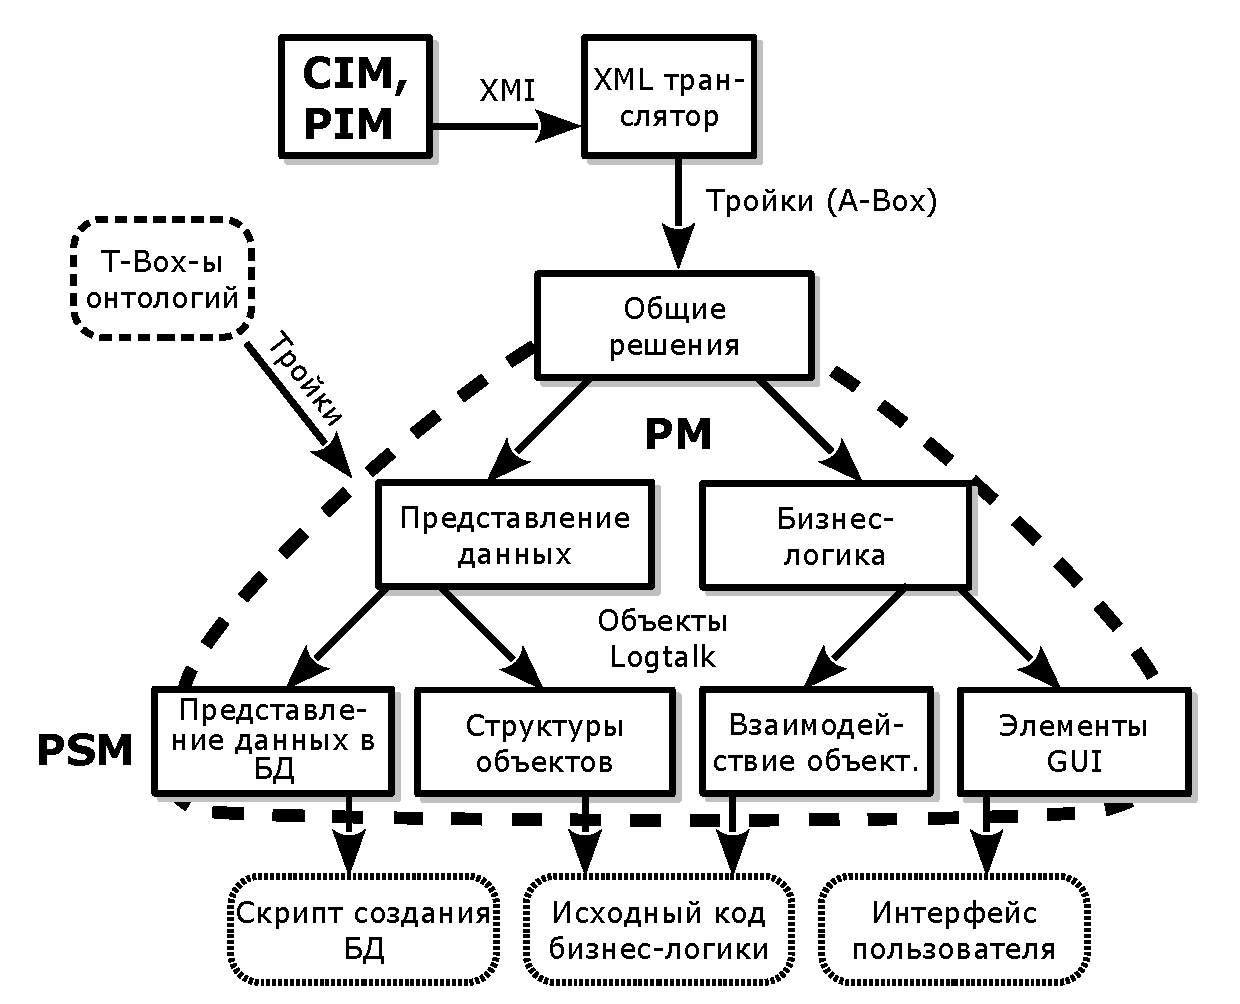
\includegraphics[width=0.9\linewidth]{qms-pics/architect_tree_pres-ru-wo-OCL.pdf}
\end{frame}

\begin{frame}
  \frametitle{Технологии и стандарты}
  \begin{itemize}
  \item Наиболее широко используемые технологии -- \textbf{ATL} и ее предшественник QVT -- стандарты OMG; поддерживают XMI$\to$XMI-преобразования; TRML.
  \item Использование ATL сдвигается на уровень CIM\footnote{Computationally independent model -- Вычислительно-независимая модель.}, например, BPMN-диаграммы преобразуются в UML (PIM\footnote{Platform independent model -- Модель, не зависящая от платформы.}); пользуется для разработки WEB-приложений, CIM представляется при помощи State- и Use case-диаграмм.
  \item Применение MDA становиться все шире, например, анализ аспектов защиты информации в распределенных приложениях; логический вывод над моделями в MDA;
  \item UML пользуется для представления CIM/PIM при моделировании онтологий; уже есть OMG-стандарт для спецификации;
  \item Спецификации на базе XML применяются для моделирования сервисов, например, WSDL, WS-BPEL;
  \item Подход MDA противопоставляется концептуальному моделированию Энна Тыугу (порождающее программирование).
  \end{itemize}

  Мы не ограничиваемся XMI на входе MDA и используем RDF.\\[0.3em]

\end{frame}

\begin{frame}
  \frametitle{Цель и задачи исследования}
  \begin{block}{}
    \textbf{Целью} исследования является создание методики разработки процедур трансформации (PD\footnote{Platform [description] model.}) в виде ОО-модулей.
  \end{block}
  \begin{columns}
    \begin{column}{0.5\linewidth}
      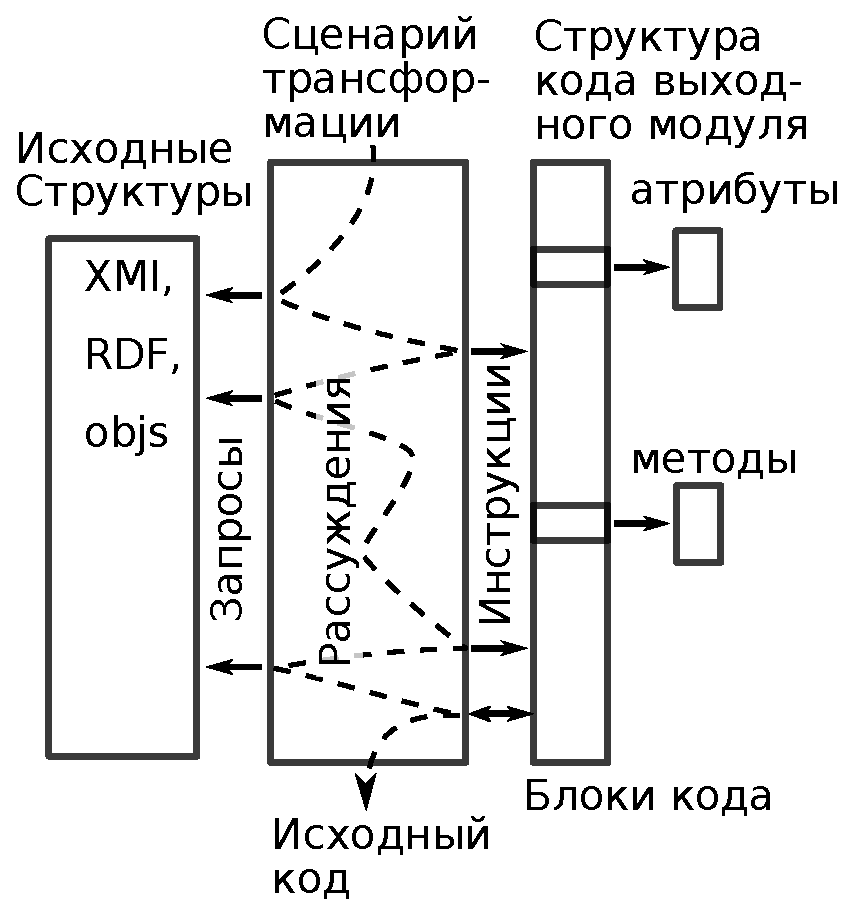
\includegraphics[width=1\linewidth]{pics/scenario-ru-wo-mothur.pdf}
    \end{column}
    \begin{column}{0.6\linewidth}
      Задачи исследования:
      \begin{itemize}
      \item Изучить синтаксические структуры Logtalk в аспекте структурирования знаний;
      \item Предложить методику представления трансформации в виде ОО-модулей;
      \item Реализовать библиотеку объектов и классов для МДА;
      \item Тестирование библиотеки на примере.
      \end{itemize}
    \end{column}
  \end{columns}
\end{frame}

\begin{frame}
  \frametitle{\href{https://logtalk.org/features.html}{Возможности макропакета LogTalk}}
  Logtalk -- декларативный ОО-язык логического программирования для ISO~Prolog (backend compiler). Обеспечивает \textbf{инкапсуляцию}, но \textbf{не позволяет хранить изменяемое состояние} (mutable state).

  \textbf{Protocols (interfaces)} задают спецификацию объекта в виде деклараций составляющих предикатов.

  \textbf{Parametric objects (and categories)}. Объекты и категории в общем случае являются сложными термами (с параметрами). Параметры задают контекст интерпретации методам без создания ненужных экземпляров.

\textbf{Prototypes and classes}. Поддерживается наследование и классов и прототипов.


\textbf{Multiple object hierarchies};

\textbf{Private, protected, and public predicates}. Можно менять области видимости при наследовании.


\textbf{Static and dynamic objects}. Статические объекты компилируются прямо в Prolog, при порождении экземпляров можно добавлять новые предикаты \emph{ad hoc}.


\textbf{Static and dynamic predicates} -- механизм инкапсулированных баз данных.
\end{frame}

\begin{frame}
  \frametitle{\href{https://logtalk.org/features.html}{Возможности макропакета LogTalk}}
\textbf{Lambda expressions}, включая каррирование (currying);

\textbf{Event-driven programming}. Можно перехватывать и фильтровать сообщения и ответы.


\textbf{Component-based programming} -- задание структур новых объектов при помощи композиции объектов и категорий. Поддержка hot patching исполняющегося кода.
\textbf{Multi-inheritance and multiple-instantiation}.

\textbf{Multi-threading programming} -- синхронная и асинхронная посылка сообщений.

\textbf{Производительность}, \textbf{Интеграция со стандартом ISO Prolog}, \textbf{Средства разработки}, включая загрузчики программ, отладчик, документирование кода, тестирование, профайлинг.

\vspace{1em}
\begin{itemize}
\item Отсутствует хороший IDE\footnote{Integrated development environment -- интегрированная среда разработки.}.
\end{itemize}
\end{frame}

\begin{frame}
  \frametitle{Инфраструктура средств MDA}
  \centering
  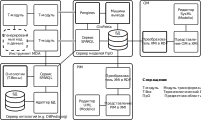
\includegraphics[width=1\linewidth]{pics/architecture-mda-lod-ext-ru.pdf}
\end{frame}

\begin{frame}[fragile]
  \frametitle{Порождение PSM класса}
  \begin{columns}
    \begin{column}{0.6\textwidth}
\begin{minted}[fontsize=\tiny]{logtalk}
:- object(direct(_Package,_LocalProf,_CodeProf)).    % Параметризованный объект для синтеза
:- public([tr/4,tr/3]).                              % определения класса
:- protected([package/1, profiles/2, profile/1]).
package(Package):- parameter(1, Package).            % Интерфейс к параметрам объекта
profile(Profile):- parameter(2, Profile).
profile(Profile):- parameter(3, Profile).
profiles(L):-
    findall(Profile, ::profile(Profile), L).
tr(class, Class, ClassID):- ::package(Package),      % Синтез класса (первый параметр метода)
    query(Package)::class(Name, ClassID),            % Запрос к структуре XMI
    create_object(Class,                             % Создание <<Класс>>
        [instantiates(class)],[],[]),
    create_object(Attributes,                        % ... <<Атрибуты>>
        [instantiates(params)],[],[]),
    create_object(Methods,                           % ...<<Методы>>.
        [instantiates(methodlist)],[],[]),
    Class::name(Name),                               % имя классу.
    forall(                                          % атрибуты
        ::tr(attribute,Attribute,ClassID,_AttrID),   % ...
        Attributes::append(Attribute) ),             % в общий список.
    forall(                                          % ...методы...
        ::tr(method, Method, ClassID, _MethodID),
        Methods::append(Method) ),
    Class::attributes(Attributes),     % Сообщить классу атрибуты.
    Class::methods(Methods).           % и методы.
tr(attribute, Attribute, ClassID, AttributeID):-     % Трансформация
    ::package(Package),                              % атрибута
    query(Package)::attribute(Name,ClassID,AttrID),
    create_object(Attribute,
        [instantiates(param)],[],[]),
    Attribute::name(Name).                           % Задать имя атрибуту.
tr(method, Method, ClassID, MethodID):-              % Трансляция метода
    ::package(Package),
    query(Package)::method(Name,ClassID,MethodID),
    create_object(Method,
    [instantiates(method)],[],[]),
    Method::name(Name).                              % Имя метода
:- end_object.                                       % Граница объекта
\end{minted}
    \end{column}
    \begin{column}{0.4\linewidth}
      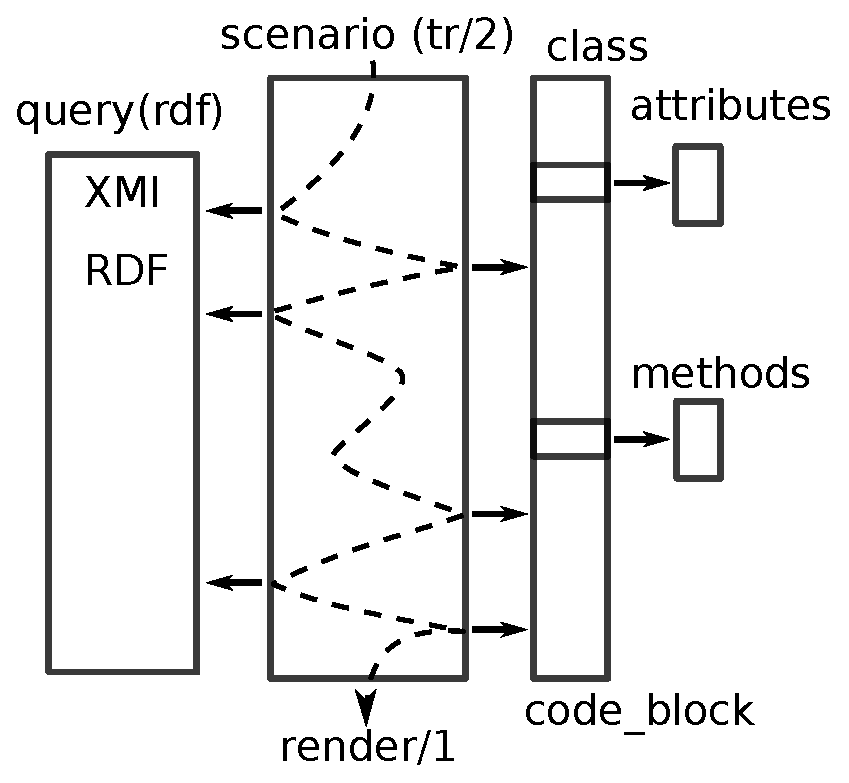
\includegraphics[width=1\linewidth]{scenario.pdf}
    \end{column}
  \end{columns}
\end{frame}

\begin{frame}[fragile]
  \frametitle{Реализация параметризованного объекта Query}
\begin{minted}[fontsize=\footnotesize{}]{logtalk}
:- object(query(_XMI)).
:- protected(xmi/1).
:- public([class/2, attribute/3, method/3]).
xmi(XMI) :- parameter(1, XMI).
class(Name, ID):-               % Распознавание класса в RDF
    ::xmi(XMI),
    XMI::rdf(ID,rdf:type,uml:'Class'),
    XMI::rdf(ID,rdfs:label, literal(Name)).
attribute(Name, ClassID, ID):-  % ...атрибута...
    ::xmi(XMI),
    XMI::graph(G),
    XMI::rdf(ClassID, G:ownedAttribute, ID),
    % XMI::rdf(ID, rdf:type, uml:'Property'),
    XMI::rdf(ID, rdfs:label, literal(Name)).
method(Name, ClassID, ID):-     % ...метода...
    ::xmi(XMI),
    XMI::graph(G),
    XMI::rdf(ClassID, G:ownedOperation, ID),
    XMI::rdf(ID, rdfs:label, literal(Name)).
:- end_object.

% query(Package)::method(Name,ClassID,MethodID),
\end{minted}
\end{frame}

\begin{frame}[fragile]
  \frametitle{Блок кода (идея почерпнута из проекта \href{https://github.com/numba/llvmlite}{llvmlite})}
  \begin{columns}
    \begin{column}{0.6\textwidth}
      \flushleft
\begin{minted}[fontsize=\tiny]{logtalk}
:- object(code_block, specializes(root)).
:- public([append/1, prepend/1, clear/0,      % Внешний интерфейс
   render/1, render_to/1, remove/1, item/1,   % объекта
   items/1 ]).
:- dynamic([item_/1]).                        % Элементы кодового блока
:- private([item_/1]).
:- protected([renderitem/2, render_to/2]).    % Методы, специализируемые
                                              % при наследовании
item(Item)   :- ::item_(Item).
items(Items) :- bagof(I, ::item(I), Items).
append(Item) :- ::assertz(item_(Item)).       % Добавить элемент в конец
prepend(Item):- ::asserta(item_(Item)).       % ...в начало
remove(Item) :- ::retract(item_(Item)).       % Удалить элемент
clear        :- ::retractall(item_(_)).       % Очистить блок кода.
render(_)    :- writef::writef("ERROR:"\      % Преобразовать блок
"Implement render/1 by a subclass!\n"), fail. % в исходный код

render_to(Stream):- ::render(List),
    ::render_to(List, Stream).
render_to(List, Stream):-
    lists::is_list(List),!,
    forall(lists::member(X,List),
       ::render_to(X, Stream)).
render_to(X,_) :- write(X),nl.
renderitem(Object, String):-    % Преобразование элемента-объекта
    current_object(Object), !,  % по умолчанию (попросить его самого
    Object::render(String).     % это сделать)
renderitem(literal(Item), String):-!, % Преобразование литерала
    atom_string(Item, String).        % (строка, число,...)
renderitem(Item, String):-            % ...строки.
    root::iswritef(String, '%q', [Item]).
:- end_object.
\end{minted}
    \end{column}
    \begin{column}{0.4\textwidth}
      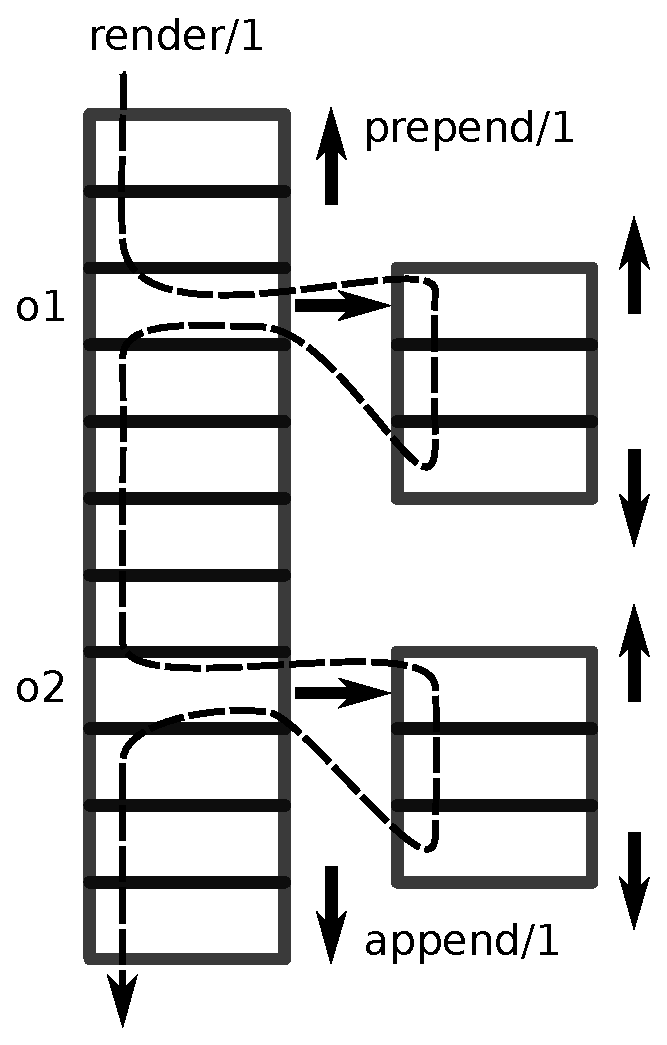
\includegraphics[width=1\linewidth]{code_block.pdf}
    \end{column}
  \end{columns}
\end{frame}

\begin{frame}[fragile]
  \frametitle{Порождение исходного кода класса Python}
    \begin{columns}
    \begin{column}{0.6\textwidth}
      \flushleft
\begin{minted}[fontsize=\tiny]{logtalk}
:- object(class, specializes(code_block),
   imports([named])). % Категория поименованных сущностей
:- public([classlist/1, methods/1, attributes/1]).
% . . . . . . . . . . . . . .
renderitem(Item, Result):-      % Использовать
    ^^renderitem(Item, Result). % унаследованный.
render(Result):-         % Генератор исходного кода,
    ^^render(Name),      % реализованный в категории
    ( ::item(classlist(List)) ->
     % . . . . . . . . . . .
        [Name]) ),
    ( ::item(attributes(Attributes))->
     % . . . . . . . . . . .
        [DefAttrList]),
      Attributes::items(InstanceAttrs),
      findall(S, ( % initialize attributes
         % . . . . . . . . .
         ), AttrAssigns),
        root::unindent,
        AttrList=[ConstructorDef|AttrAssigns];
         % . . . . . . . . .
        AttrList=[ConstructorDef, Pass] ),
    ( ::item(methods(Methods))-> % Если есть ...
      Methods::render(MethodList);
      MethodList=[] ),
    lists::append(AttrList,MethodList,StringList),
    root::unindent, Result=[Signature|StringList].
:- end_object.
\end{minted}
    \end{column}
    \begin{column}{0.4\linewidth}
      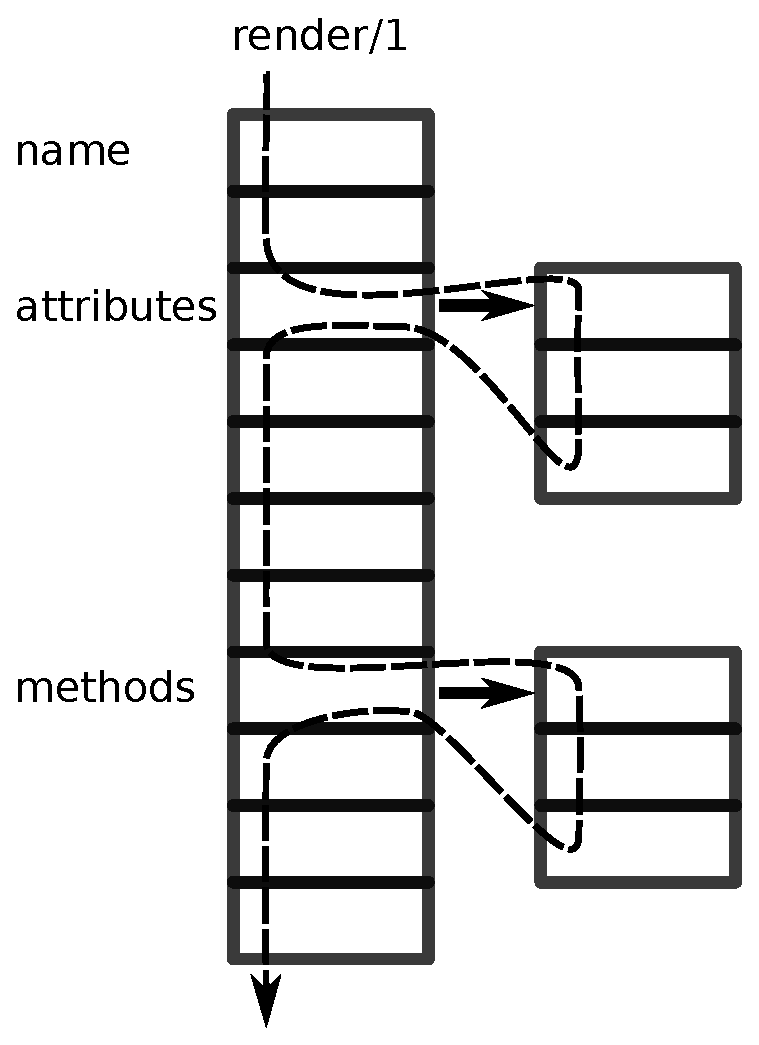
\includegraphics[width=1\linewidth]{code_block_class.pdf}
        Класс-генератор -- это специализация кодового блока.
    \end{column}
  \end{columns}
\end{frame}

\begin{frame}[fragile]
  \frametitle{Категории}
  Категория поименованных сущностей
\begin{minted}{logtalk}
:- category(named).
:- public([name/1, render/1]).
:- protected([renderitem/2]).
name(Name):- ::prepend(name(Name)).
renderitem(name(Name), String):-!, atom_string(Name, String).
render(String):-  % Как генерировать код
    ::item(name(Name)),
    ::renderitem(name(Name), String).
:-end_category.
\end{minted}
Категория поименованных сущностей, имеющих тип
\begin{minted}{logtalk}
:- category(namedtyped, extends(named)).  % Дополняем категорию <<named>>
:- public([type/1,render/2, separator_option/2,list_separator/1]).
:- protected([renderitem/2]).
type(Type):- ::append(type(Type)).
renderitem(Item, String):-
    ^^renderitem(Item, String),!.
renderitem(type(Type),String):-!,
    ::list_separator(Separator),
    writef::swritef(String, '%w%w', [Separator, Type]).
render(Middle, String):-
    ^^render(SName),
    (   ::item(type(Type)) ->
        ::renderitem(type(Type), SType),
        string_concat(SName, Middle, _1),
        string_concat(_1, SType, String) ;
        SName = String  ).
render(String):-  ::render("", String).

list_separator(Separator):-
    ::separator_option(Name, Default),!, % Глобальные настройки
    root::option(Name, Separator, Default).
:- end_category.

\end{minted}
\end{frame}

\begin{frame}[fragile]
  \frametitle{Доступ к сервисам SPARQL}

  \begin{columns}
\begin{column}{0.5\textwidth}
\begin{minted}[fontsize=\scriptsize]{logtalk}
:- category(sparql).
:- public(query/2).
query(Pattern,Parameters,Row):-
    prepare(Pattern,Parameters,Query),
    server(Host,Port,Path),
    sparql_query(Query, Row,
        [host(Host),port(Port),path(Path)]).
:- protected(server/3).  % нужно реализовать
                         % в подклассе.
:- protected(prepare/3). % Подготовить строку
% . . . . . . . . . .    % запроса.
:- end_category.

:- object(dbpedia, extends(sparql)).
:- protected(server/3).
server('dbpedia.org',80,'/sparql').
:- public(entity_name/2).
entity_name(Entity,Language,Name):-
    query('select ?name where { '
          ' %w rdfs:label ?name. '
          'FILTER langMatches( lang(?label),'
          ' "%w" )}', [Entity, Language],
          row(Name)).
:- end_object.

% ?- dbpedia::entity_name(dbr:'Passport', 'ru', Name).
\end{minted}
\end{column}
\begin{column}{0.5\textwidth}
  \flushright
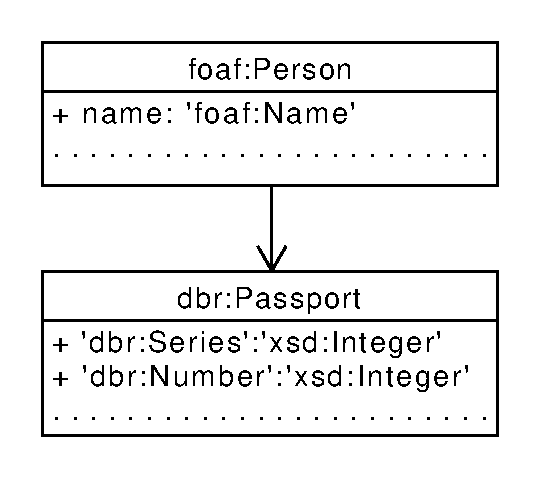
\includegraphics[width=0.8\linewidth]{simple-diag.pdf}
\end{column}
\end{columns}
\end{frame}


\begin{frame}
  \frametitle{Порождение модулей Rapidminer по исходному коду Mothur}
  \begin{center}

  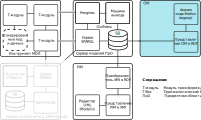
\includegraphics[width=1\linewidth]{pics/architecture-mda-lod-ext-ru-rapidminer.pdf}

  \end{center}
\end{frame}

\begin{frame}[fragile]
  \frametitle{Пример синтезированного исходного кода модуля}
\begin{minted}{java}
package com.rapidminer.ngs.operator;

. . . . . . . . . . . .
import com.rapidminer.parameter.*;

public class MothurRemoveOtusOperator extends MothurGeneratedOperator {

	private InputPort accnosInPort = getInputPorts().createPort("accnos");
	. . . . . . . . . . . .
	private InputPort sharedInPort = getInputPorts().createPort("shared");
	private OutputPort constaxonomyOutPort = getOutputPorts().createPort("constaxonomy");
	. . . . . . . . . . . .
	private OutputPort sharedOutPort = getOutputPorts().createPort("shared");
	private static final String LABEL_LABEL = "label:";
	. . . . . . . . . . . .
	private static final String OUTPUTDIR_LABEL = "outputdir:";

	public MothurRemoveOtusOperator (OperatorDescription description) {
		super(description);  // NOTE: Auto-generated constructor stub
	}

	@Override
	public void doWork() throws OperatorException {
		super.doWork();
		clearArguments();
		FileNameObject accnosFile = accnosInPort.getData(FileNameObject.class);
		addArgument("accnos",accnosFile.getName());
		. . . . . . . . . . . .
		executeMothurCommand();
		. . . . . . . . . . . .
		otucorrOutPort.deliver(new FileNameObject(fileName+".otucorr","otucorr"));
		sharedOutPort.deliver(new FileNameObject(fileName+".shared","shared"));
	}

	@Override
	public List<ParameterType> getParameterTypes() {
		List<ParameterType> parameterTypes = super.getParameterTypes();
		parameterTypes.add(new ParameterTypeString(LABEL_LABEL, "TODO: Add description", "", true));
		. . . . . . . . . . . .
		return parameterTypes;
	}
	. . . . . . . . . . . .
}
\end{minted}
\end{frame}
\begin{frame}
  \frametitle{Представление NGS в виде диаграммы потоков данных}
  \begin{columns}
    \begin{column}{0.6\textwidth}
      \begin{raggedright}
        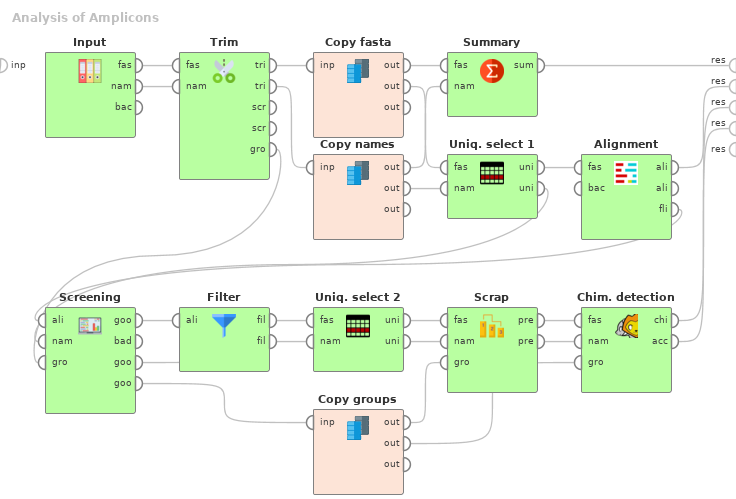
\includegraphics[width=1\linewidth]{Dataflow-color-en.png}
      \end{raggedright}
    \end{column}
    \begin{column}{0.4\textwidth}\footnotesize
      \begin{tabular}{ll}
        Термин & Расшифровка \\
        \hline
        NGS & Секвенирование нового\\ & поколения\\
        Ампликон & Часть ДНК или РНК, \\
               & скопированная много \\
               & раз \\
        Mothur & Прикладной пакет для\\ & исследований в NGS \\
        Rapidminer & Инструмент визуально- \\
             & го моделирования \\
             & вычислительных \\
             & процессов
      \end{tabular}
      ${}$\\[1em]
      Зеленые блоки -- модули Mothur. Остальные -- модули Rapidminer.
    \end{column}
  \end{columns}
  \vspace{1em}
  Сгенерировано \textbf{145 классов Java} для каждой операции Mothur, а также \textbf{два файла} с описанием структуры пакета NGS для Rapidminer (XML).
\end{frame}


\begin{frame}
  \frametitle{Результаты}
  Общее впечатление от применения LogTalk:
  \begin{itemize}
  \item Logtalk и RDF -- это гибкая, достаточно универсальная и удобная в реализации инфраструктура MDA;
  \item Самые замечательные средства реализации -- это обрамление запросов в предикаты Prolog и инкапсуляция правил в объекты LogTalk;
  \item Не все структуры LogTalk задействованы в реализации: можно разработать и более специфические методики программирования, например, с использованием перехвата сообщений.
  \end{itemize}
  Технические сопутствующие проблемы:
  \begin{itemize}
  \item Самые простые задачи требуют больших усилий, например, обработка текста: преобразование идентификатора в CamelCase;
  \item Достаточно трудно найти подходящую онтологию в Интернет, но это в далекой перспективе более продуктивно, чем разрабатывать свою;
  \item Prolog и LogTalk не являются популярными языками: приходится самому вырабатывать приемы программирования.
  \end{itemize}
\end{frame}

\begin{frame}
  \frametitle{Заключение}
  К настоящему времени получены следующие результаты:
  \begin{itemize}
  \item Разработана методика представления визуальных моделей ПО и входных данных MDA.
  \item Выработан ряд приемов программирования модулей трансформации на ОО-языке LogTalk.
  \item Реализована $\alpha$-версия библиотеки трансформации.
  \item Разработанный инструментарий протестирован на двух задачах: Mothur $\to$ Rapidminer и синтез протокола обмена с контрольно-кассовой машиной.
  \end{itemize}
  Направления дальнейшего развития:
  \begin{itemize}
  \item Обеспечить семантическую разметку интерфейсов и выходных документов на основе логического вывода семантики публикуемых данных.
  \item Разработать методики программирования трансформации, минимизируя количество динамических объектов.
  \item Создать профессиональную среду разработки программного обеспечения из имеющегося прототипа.
  \item Разработать методику синтеза реализаций протоколов обмена информацией (OSPFv6) и различных ORM.
  \end{itemize}
\end{frame}


\begin{frame}
  \vfill
  \begin{center}
    {\Huge Спасибо за внимание!}
  \end{center}
  \vfill
  Исходный код (без документации) доступен на github.com: \url{https://github.com/isu-enterprise/icc.xmitransform}, \url{https://github.com/eugeneai/icc.mothurpim}.
\end{frame}


\begin{frame}
  \frametitle{Диаграмма BPMN2.0}
  BPMN -- Business process modeling notation
  \centering
    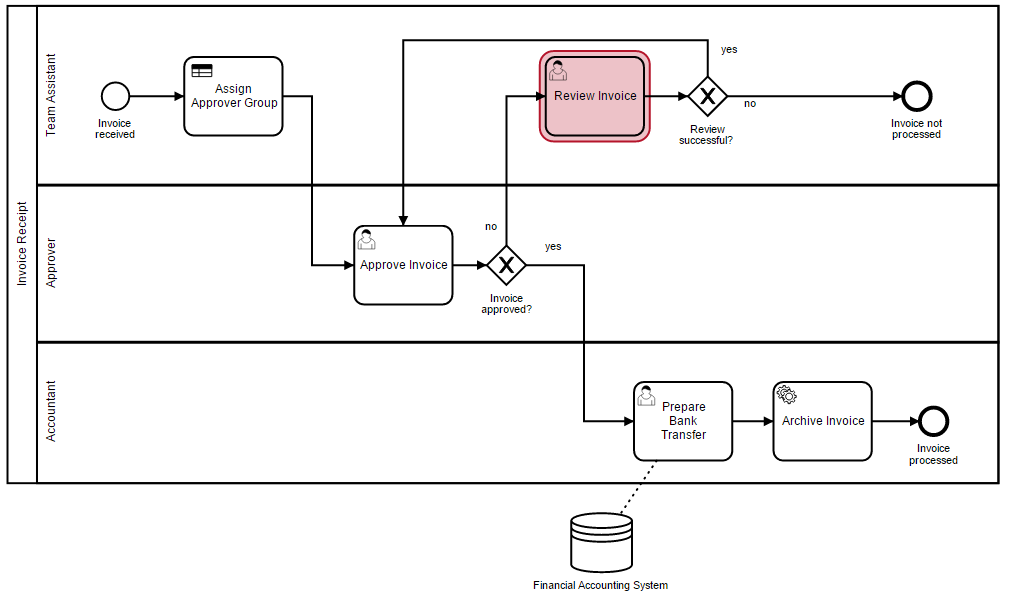
\includegraphics[width=1\linewidth]{qms-pics/bpmn.png}
\end{frame}
\begin{frame}
  \frametitle{Диаграмма CMMN1.1}
  CMMN -- Case management model and notation
  \centering
    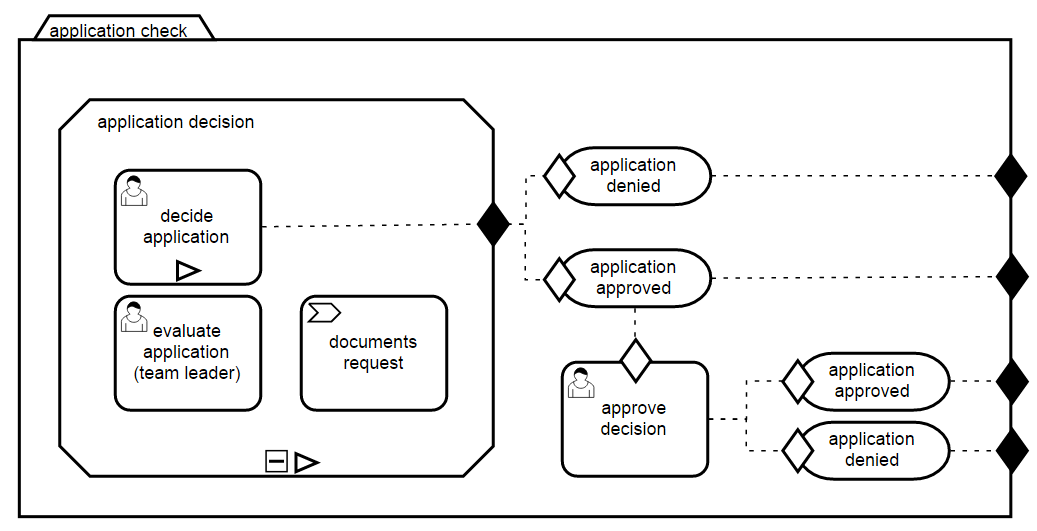
\includegraphics[width=1\linewidth]{qms-pics/cmmn.png}
\end{frame}

\end{document}

%%% Local Variables:
%%% mode: latex
%%% TeX-master: t
%%% End:
